\newcommand{\largeur}{0.5}
\newcommand{\hauteur}{1.5}
\newcommand{\rayon}{0.075cm}
\newcommand{\ytext}{-1}
\newcommand{\ytexth}{3*\hauteur+2.5}
\newcommand{\dlayer}[3]{ \draw[fill=#3] (#1,#2) rectangle (#1+\largeur,#2+\hauteur); %
  \foreach \y in {0.25,0.5,...,1.25}{ \draw[fill=black] (#1+\largeur/2,#2+\y) circle (\rayon);};%
}
\newcommand{\greenhc}{\color{green!50!black}}
\newcommand{\hiddenl}{\greenhc\seq{h}_t}



\newcommand{\wcontext}{\mathbf{h}}
\renewcommand{\mydot}[2]{\left\langle {#1} , {#2} \right\rangle} % scalair product

% \newcommand{gcolor}{red!40}
% \colorlet{gcolor}{green!60!black} % color for good word
\colorlet{gcolor}{blue} % color for good word
\colorlet{hcolor}{orange} % color for context 
\newcommand{\gw}{{\color{gcolor}\ws}} % good word
\newcommand{\gwi}{{\color{gcolor}\ws_i}} % good word
\newcommand{\whscore}{\ensuremath{s_{\params}({\gwi},{\color{hcolor}\wcontext})}}

\begin{frame}{A word prediction ``game''}
  \begin{center}
    $P( \ws_i = \textrm{?}  | \underbrace{\mathbf{\ws}_{1}^{i-1}
    }_{\color{orange}\textrm{context: }\mathbf{h}})\ \ \ \ \rightarrow\ \ \ $
    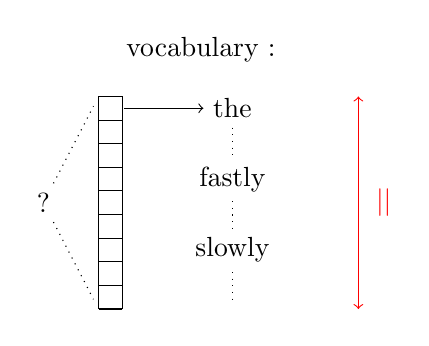
\begin{tikzpicture}[baseline=1.22cm]
      %%%%%%%%%%%%%%% 1st
      \node (pred) at (-1, 1.35) {?};

      { \node (the) at (1.4,2.55) {the}; }

      { \node (bas) at (-.3, 0) {}; \node (haut) at (-.3, 2.7) {};
        \draw[step=.3] (-.3, 0) grid (0, 2.7); \draw[dotted] (pred) --
        (bas); \draw[dotted] (pred) -- (haut);
        % 
        \node (voc) at (1,3.3) {vocabulary $\vocab$:}; \node (the0) at
        (-0.1,2.55) {};
        
        % 
        \node (fastly0) at (-0.1,1.65) {}; \node (fastly) at
        (1.4,1.65) {fastly}; \node (slowly0) at (-0.1,0.75) {}; \node
        (slowly) at (1.4,0.75) {slowly};

        \node (basmot) at (1.4,0) {}; \draw[->] (the0) -- (the);
        \draw[dotted] (the) -- (fastly); \draw[dotted] (fastly) --
        (slowly); \draw[dotted] (slowly) -- (basmot);

        \draw[<->,red] (3,2.7) -- (3,-0);
        \node[anchor=west,red] (V) at (3.1,1.35) {$|\vocab|$};
      }
    \end{tikzpicture}
  \end{center}
  \begin{itemize}
  \item $\vocab$ is a finite set of words 
  \item A probability distribution over $\vocab$, $\forall\
    {\color{orange}\mathbf{h}}$

  \item ${\color{orange}\mathbf{h}}=[\textrm{time}, \textrm{goes},
    \textrm{by}, \textrm{so} ]$
  \end{itemize}
\end{frame}


\begin{frame}
  \frametitle{Language model / Generative sequence model}
  \begin{block}{Applications}
    Automatic Speech Recognition, Machine Translation, OCR, ... 
  \end{block}

  \begin{block}{The goal}
    Estimate the \textbf{non-zero} probability of a word sequence given a vocabulary 
    $$
    P(\wsseq{1}{L}) = P(\ws_1, \ws_2, ... \ws_L) = \prod_{i=1}^L P(\ws_i | \wsseq{1}{i-1}),\ \ \forall i , \ws_i \in \vocab
    $$

    with the \textbf{\ngram assumption}:
    $$
    P(\wsseq{1}{L}) = \prod_{i=1}^L P(\ws_i | \wsseq{i-n+1}{i-1}),\ \ \forall i , \ws_i \in \vocab,
    $$

    in the \textbf{recurrent} way 
    $$ P(\ws_i | \wsseq{1}{i-1})$$
  \end{block}
\end{frame}


\begin{frame}{Challenges}
  \begin{itemize}
  \item Share knowledge among similar words
    \begin{center}
      \begin{tabular}{l|r}
        you {\color{red}go} to {\color{green}London} &you go to {\color{blue}Montelimar}\\
        you {\color{red}went} to {\color{green}London} &you went to {\color{blue}Montelimar}
      \end{tabular}
    \end{center}
  \item Keep/skip what is meaningful/meaningless
    \begin{center}
      Dr. Janet who visited us last year Smith talks about ...
    \end{center}
  \item Long distance dependancies
    \begin{center}
      to greatly play \textbf{chess} he wants to  have a nice \textbf{board}\\
      to greatly play \textbf{music} he wants to buy a new  \textbf{keyboard}
    \end{center}
  \end{itemize}
\end{frame}


\begin{frame}{Count-based language model}
  \framesubtitle{\ngram LM}
  \begin{align*}
    P(\wsseq{1}{L}) &= \prod_{i=1}^L P(\ws_i | \wsseq{i-n+1}{i-1}),\ \
                      \forall i , \ws_i \in \vocab,\\
    P_{ML}(\ws_i | \wsseq{i-n+1}{i-1}) &=
                                         \frac{c(\wsseq{i-n+1}{i})}{c(\wsseq{i-n+1}{i-1})}
  \end{align*}
  \begin{itemize}
  \item Very inefficient ! 
  \item How to deal with zero counts in the denominator ? 
  \item In the numerator ? 
  \item Zero counts are the most frequent case. 
  \item[$\rightarrow$] smoothing~\cite{Kneser95Improved,Chen98Empirical}
  \end{itemize}
\end{frame}


\begin{frame}{Estimate $n$-gram probabilities in a continuous space}
  Introduced in~\cite{Bengio01,Bengio03aneural} 
  \begin{block}{In a nutshell}
    \begin{enumerate}
    \item associate each word with a continuous feature vector
    \item express the probability function of a word sequence in terms
      of the feature vectors of these words
    \item learn simultaneously the feature vectors and the parameters
      of that probability function.
    \end{enumerate}
  \end{block}
  \begin{block}{Why should it work ?}
    \begin{itemize}
    \item  "similar" words are expected to have a similar feature vectors
    \item  the probability function is a smooth function of these
      feature values
      \begin{itemize}
      \item  a small change in the features will induce a small
        change in the probability
      \item Remember: \textsc{London} and \textsc{Montelimar}
      \end{itemize}
    \end{itemize}
  \end{block}
\end{frame}


\begin{frame}{Word (discrete symbols) embeddings}
  \begin{block}{One-hot encoding}
    \begin{center}
      \begin{displaymath}
        \textrm{Assume the vocabulary:~~~~~~~~~}
        \left.
          \begin{array}{l}
            the\\
            \mathbf{this}\\
            awesome\\
            ...\\
            great
          \end{array} 
        \right\} \rightarrow \x = 
        \left( 
          \begin{array}{c}
            0\\
            \mathbf{1}\\
            0\\
            ...\\
            0
          \end{array}
        \right)
      \end{displaymath}
    \end{center}
  \end{block}
  \begin{block}{Look-up table}
    \begin{center}
      \begin{displaymath} % 
        \underbrace{\wmatrix}_{\textrm{\tiny Look-up table}} \times \x = 
        \left(
          \begin{array}{ccccc}
            \vdots &\vdots &\vdots &\vdots &\vdots \\
            \wvector_{the} & \wvector_{this} & \wvector_{awesome} & \cdots &  \wvector_{great}\\
            \vdots &\vdots &\vdots &\vdots &\vdots \\
          \end{array} 
        \right) \times 
        \left( 
          \begin{array}{c}
            0\\
            \mathbf{1}\\
            0\\
            0\\
            0
          \end{array} 
        \right)  = \wvector_{this} 
      \end{displaymath}
    \end{center}
  \end{block}
\end{frame}


\begin{frame}
  \frametitle{Word embeddings}
  \begin{block}{Definitions}
    \begin{itemize}
    \item A continous vector associated to each word (discrete symbol): its
      \important{embedding}. 
    \item The matrix $\wmatrix$ is called the \important{look-up
        table} and store the word embeddings. 
    \end{itemize}
  \end{block}
  \begin{itemize}
  \item The term \textit{look-up} comes from the real operation\\
    $\wmatrix\times\x$ is only theoritical !
  \item No computational cost, only storage and trainability
    challenge\\ (enough observations for each words, ...) 
  \item Pre-trained, fine-tuned, ... 
  \end{itemize}
\end{frame}



\begin{frame}{Neural language model basics}
  \begin{columns}
    %%%%%%%%%%%%%%%%%%%%%%%%%%%%%%%%%%%%%%%%%%%%%%%%%%%%%%%%%%%% 
    \column{0.5\textwidth}
    \begin{center}
      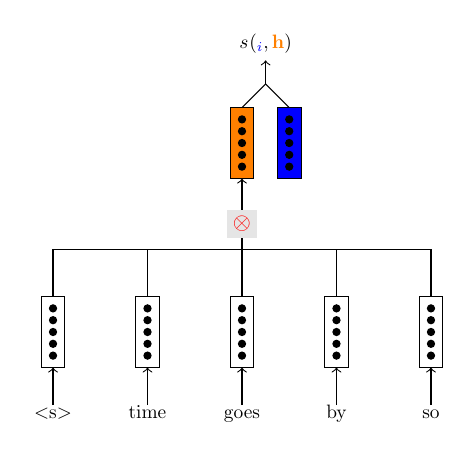
\begin{tikzpicture}[scale=0.6,every node/.style={scale=0.7}]
        \node[anchor=mid] (time) at (0+\largeur/2,\ytext){$<$s$>$};
        \node[anchor=mid] (goes) at (2+\largeur/2,\ytext) {time};
        \node[anchor=mid] (by) at (4+\largeur/2,\ytext) {goes};
        \node[anchor=mid] (so) at (6+\largeur/2,\ytext) {by};
        \node[anchor=mid] (dots) at (8+\largeur/2,\ytext) {so};

        % words embeddings
        \uncover<2->{
          \foreach \x in {0,2,...,8}{\dlayer{\x}{0}{white}};
          % links from text to embeddings
          \foreach \x in {0,2,...,8}{\draw[->]
            (\x+\largeur/2,\ytext+0.2) -- (\x+\largeur/2,0);};

        }
        \uncover<3->{
          % links from embeddings to hidden layers
          \foreach \x in {0,2,...,8}{\draw
            (\x+\largeur/2,0+\hauteur) --
            (\x+\largeur/2,\hauteur+1);};
          % horizontal
          \draw (0+\largeur/2,\hauteur+1) --
          (8+\largeur/2,\hauteur+1);
          % merge arrow
          \draw[->] (4+\largeur/2,1+\hauteur) --
          (4+\largeur/2,\hauteur+2.5);
          % Composition operator
          \node[anchor=mid,fill=gray!20] (merge) at
          (4+\largeur/2,\hauteur+ 1.5)
          {\color{red}\large$\boldsymbol{\otimes}$};
          % Context vector
          \dlayer{4}{\hauteur+2.5}{hcolor}
        }
        \uncover<4->{
          % Output vector / embeddings
          \dlayer{5}{\hauteur+2.5}{gcolor}
          % output arrows
          \draw[-] (4+\largeur/2,2*\hauteur+2.5) --
          (4.5+\largeur/2,2*\hauteur+3) ;
          \draw[-] (5+\largeur/2,2*\hauteur+2.5) --
          (4.5+\largeur/2,2*\hauteur+3) ;
          \draw[->] (4.5+\largeur/2,2*\hauteur+3) --
          (4.5+\largeur/2,2*\hauteur+3.5) ;
          % output score
          \node[anchor=south] (s) at (4.5+\largeur/2,2*\hauteur+3.5)
          {$\whscore$};
        }
      \end{tikzpicture}
    \end{center}
    %%%%%%%%%%%%%%%%%%%%%%%%%%%%%%%%%%%%%%%%%%%%%%%%%%%%%%%%%%%% 
    \column{0.5\textwidth}
    \small
    To estimate $P(\gwi | \wsseq{1}{i-1})$:
    \begin{itemize}
    \item<2-> each $\ws_i \in \wsseq{1}{i-1} \rightarrow$ embedded
    \item<3-> build a context vector $\color{hcolor}\wcontext$ for $\wsseq{1}{i-1}$
    \item<4-> the score of  a target word $\gwi$:
      $$\whscore$$
    \end{itemize}
    \uncover<5->{\vspace{-4ex} Details:
      \begin{itemize}
      \item $\params$: all the parameters
      \item $\whscore=\mydot{\color{gcolor}\ws_i}{\color{hcolor}\wcontext} $
      \item The probability distribution: 
        \begin{align*}
          P(\ws_i | \wsseq{1}{i-1}) &= \frac{\exp(\whscore)}{Z({\color{hcolor}\wcontext})}\\
          Z({\color{hcolor}\wcontext}) &=  \sum_{\ws\in\vocab} \exp(s_{\params}(\ws,{\color{hcolor}\wcontext}))
        \end{align*}
      \item What is  {\color{red}\large$\boldsymbol{\otimes}$} ? 
      \end{itemize}
      \vfill
    }
    
  \end{columns}
\end{frame}



\begin{frame}{Estimate the $n$-gram probability}
  \begin{columns}
    \begin{column}{0.6\textwidth}
      % \begin{beamercolorbox}[center,rounded=true,sep=0.5ex]{postit}
      %   Estimate the \textit{n-gram} probability in terms of the
      %   sequence of feature vectors instead of multinomials
      % \end{beamercolorbox}\pause
      \begin{block}{The program}
        \begin{itemize}
          % \item Associate each word with feature vector
          %   in a continous space.\pause
        \item<1-> Given  the history expressed as a  feature vector :
          {$\mathbf{v}$} (only the $n-1$ last words)
        \item<2-> Create a feature vector for the next word: $$ \mathbf{h} = f(\mathbf{W}_{vh} \mathbf{v}) $$
        \item<3-> For all words given the history:
          \begin{align*}
            \mathbf{o} &= f(\mathbf{W}_{ho} \mathbf{h}) \\
            P(\ws_i|\wsseq{i-n+1}{i-1}) &= \frac{\exp(o_{w_i})}{\sum_{\ws
                                          \in \vocab}\exp(o_{w_i}) }
          \end{align*}
          % \item<4-> All the parameters must be learnt ($\mathbf{R}, \mathbf{W_{vh}}, \mathbf{W_{ho}} $)
        \end{itemize}
      \end{block}
    \end{column}
    \begin{column}{0.4\textwidth}
      % \only<1>{\includegraphics[height=0.8\textheight]{./figs/cslm_1.pdf}}
      \only<1|handout:0>{\includegraphics[width=\textwidth]{../figs/cslm_2.pdf}}
      \only<2|handout:0>{\includegraphics[width=\textwidth]{../figs/cslm_3.pdf}}
      \only<3-|handout:1>{\includegraphics[width=\textwidth]{../figs/cslm_4.pdf}}
    \end{column}
  \end{columns}
\end{frame}


\begin{frame}{Learning and inference issues}
  \begin{block}{Training objective and gradients}
    \begin{align*}
      \fullloss &=  \sum_{(\ws,\wcontext) \in \dataset}  \log P_{\params}(\ws|\wcontext) \\
      \frac{\partial\fullloss }{ \partial\params} &=  \frac{\partial  \whscore} {\partial \params} - \sum_{\ws'\in\vocab} P_{\params}(\ws'|\wcontext)  \frac{ \partial  s_{\params}(\ws',\wcontext)}{\partial \params}
    \end{align*}
    % The vocabulary size $|\vocab| \Rightarrow$
    \begin{itemize}
    \item Large $|\vocab|$ is prohibitive
    \item Prediction in a high dimensional space
    \end{itemize}
  \end{block}
  \begin{block}{Solutions}
    \begin{itemize}
    \item Structured output~\cite{Le10Training,Le11Soul,Le13SOUL}
    \item New training criterion~\cite{Mnih12Fast,labeau17NCE}
    \end{itemize}
  \end{block}
\end{frame}


